\subsection{Forward Burgers PINN: one versus four loss components}
\label{sec:burgers-forward-experiment}

The forward problem compares one aggregated component with four resolved
components at \(\alpha=1/2\), under the same momentum and adaptive scaling
rules. The inverse problem then adds sparse observations and an unknown
viscosity.

We consider the viscous Burgers equation
\begin{equation}
  u_t+uu_x-\nu u_{xx}=0,
  \qquad (x,t)\in[-1,1]\times[0,1],
  \qquad \nu=0.01,
  \label{eq:burgers-forward-pde}
\end{equation}
with initial and boundary conditions
\begin{equation}
  u(x,0)=-\sin(\pi x),
  \qquad u(-1,t)=u(1,t)=0.
  \label{eq:burgers-forward-data}
\end{equation}
The PINN is a tanh network with six hidden layers of width 64 and 21,057
trainable parameters. Every run uses 10,000 fixed scrambled Sobol collocation
points \cite{sobol1967,owen1997}, 256 initial points, 256 time points on each
boundary, and 10,000
independent validation collocation points.  The relative solution error is
evaluated against a grid-refined backward differentiation formula (BDF)
method-of-lines reference on a
\(256\times101\) space--time grid.

Let \(r_f=u_t+uu_x-\nu u_{xx}\).
For sampled values \(w_1,\ldots,w_N\), we use
\(\operatorname{MSE}(w)=N^{-1}\sum_{j=1}^N w_j^2\).
The common PINN task objective is
\begin{subequations}
\label{eq:burgers-forward-losses}
\begin{align}
  E_{\rm res}
  &=\frac12\operatorname{MSE}(r_f),\\
  E_{\rm bc}
  &=\frac14\left[
    \operatorname{MSE}(u(-1,t))+
    \operatorname{MSE}(u(1,t))\right],\\
  E_{\rm ic}
  &=\frac12\operatorname{MSE}(u(x,0)+\sin(\pi x)),\\
  F_{\rm task}
  &=E_{\rm res}+E_{\rm bc}+E_{\rm ic}.
\end{align}
\end{subequations}
All methods use the weight-decay coefficient \(\lambda=10^{-6}\).  For
PB--SAV, weight decay is represented by the explicit component
\begin{equation}
  F_{\rm reg}(\theta)
  =F_{\rm task}(\theta)+E_{\rm wd}(\theta),
  \qquad
  E_{\rm wd}(\theta)=\frac{\lambda}{2}\norm{\theta}^2.
  \label{eq:burgers-forward-regularized}
\end{equation}
We report \(F_{\rm task}\), which is common to all methods, as the primary
optimization quantity.

We compare heavy-ball gradient descent, AdamW, adaptive PB--SAV with momentum
using one
aggregate component, and the same PB--SAV method using the four components
\(E_{\rm res}\), \(E_{\rm bc}\), \(E_{\rm ic}\), and \(E_{\rm wd}\).
The total SAV shift is \(10^{-12}\).  One quarter is assigned to weight decay,
and the remainder is distributed among the three physical terms in proportion
to their sample counts.
A seed-0 pilot selects learning rates from the task objective only.  The
selected rates are \(10^{-2}\) for heavy-ball gradient descent and
\(10^{-3}\) for AdamW and both PB--SAV variants.  Reported runs use 10,000
updates at the paired seeds \(42, 2273, 2669, 5439, 8041\).

\begin{figure}[t]
  \centering
  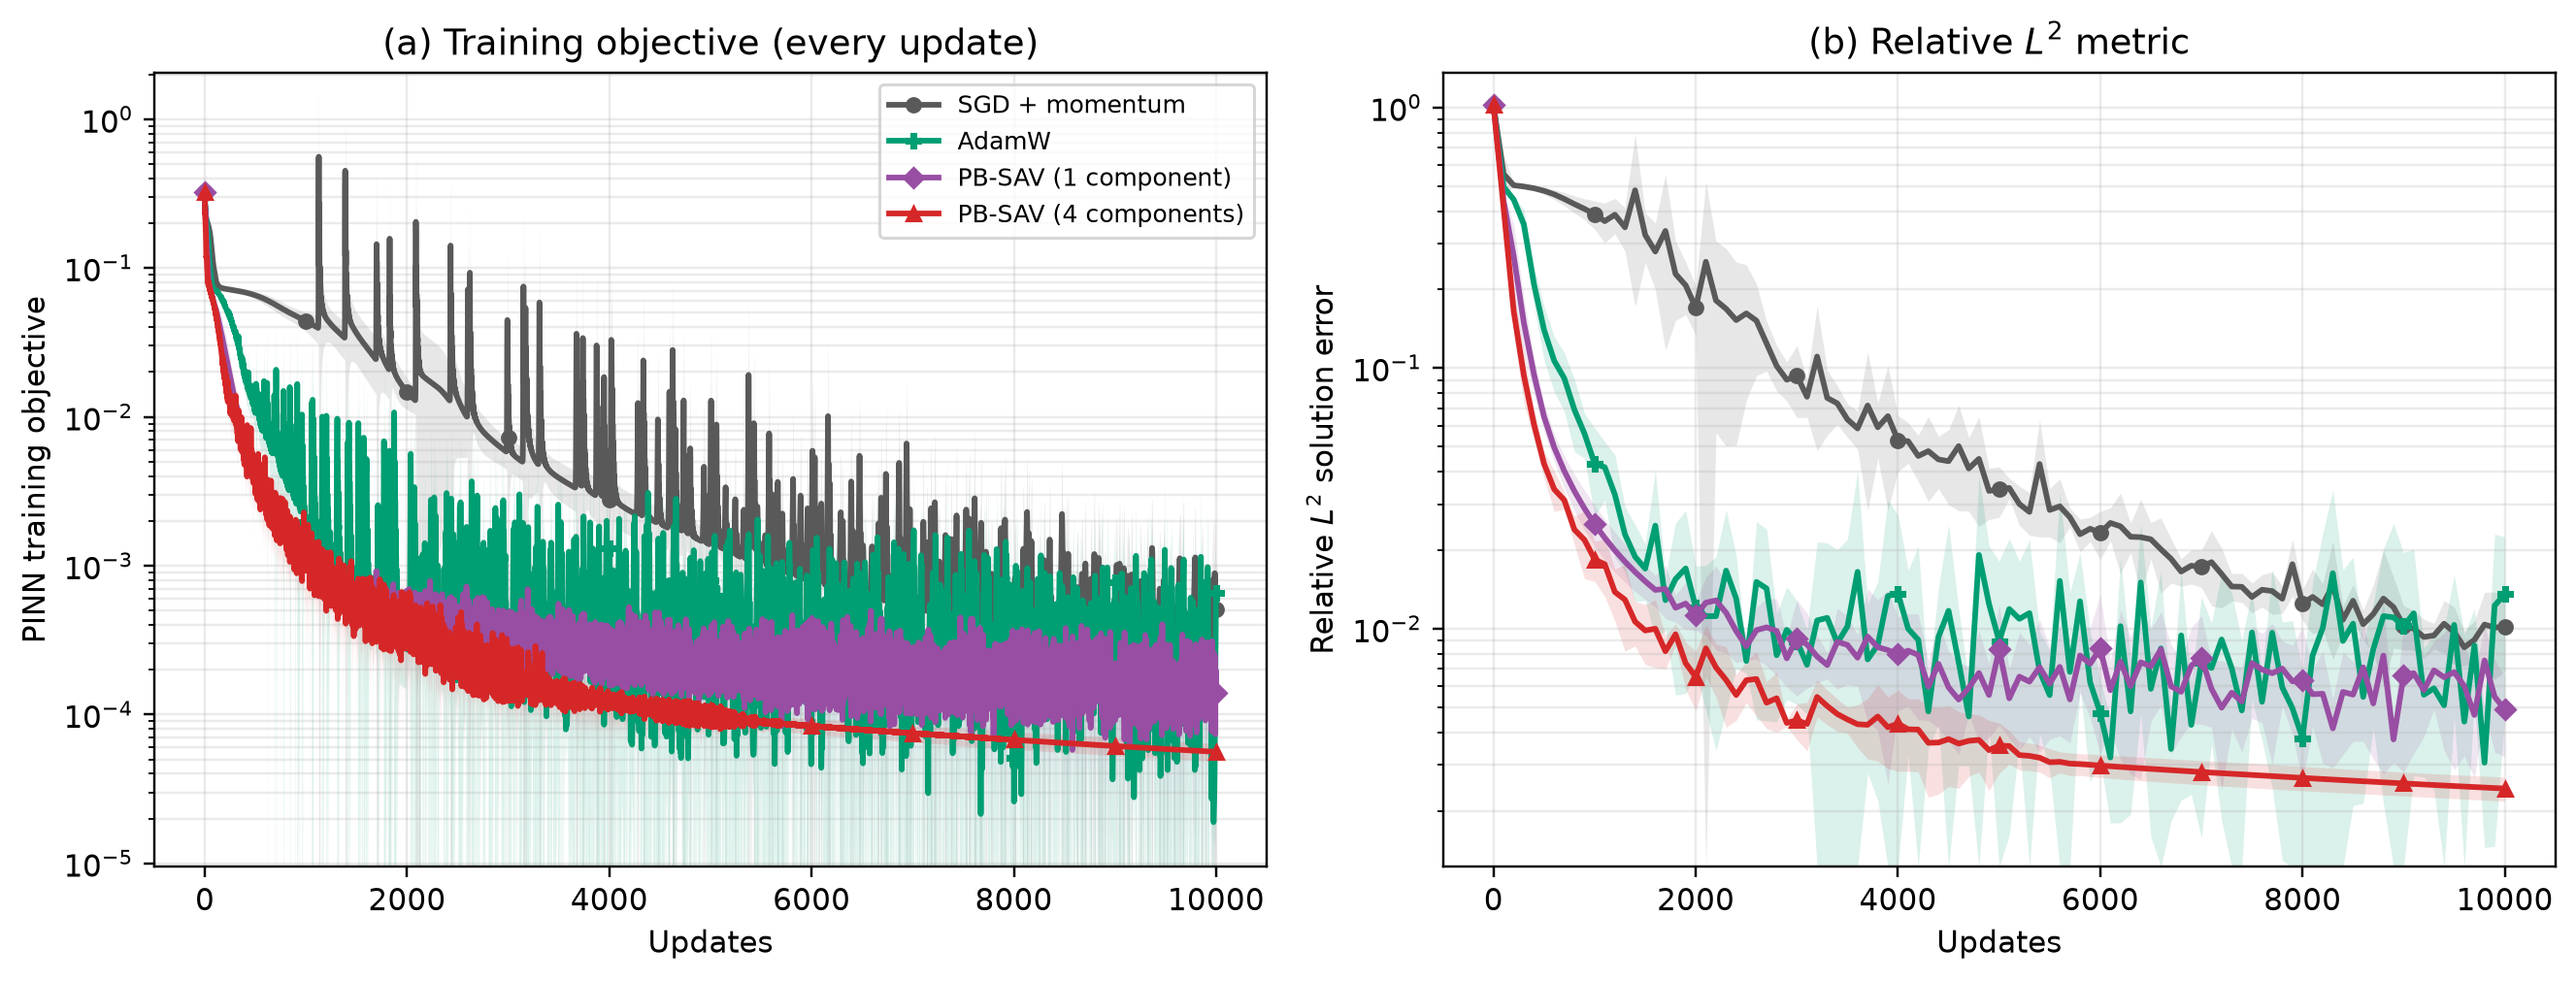
\includegraphics[width=\textwidth]{burgers_forward_optimizer_performance.png}
  \caption{Five-seed comparison for the forward Burgers PINN.  (a) Mean common
  task objective, recorded at every update, and (b) mean relative \(L^2\)
  solution error.  Shaded regions show one sample standard deviation.}
  \label{fig:burgers-forward-results}
\end{figure}

\begin{table}[t]
\centering
\caption{Forward Burgers results after 10,000 updates over five paired seeds.
For each seed, the tail mean and coefficient of variation (CV) are computed
over the final 2,000 updates; the table reports their mean \(\pm\) sample
standard deviation across seeds.  Here
\(\mathrm{CV}=100s_{\rm tail}/\bar F_{\rm tail}\).  Best mean values are
bold.}
\label{tab:burgers-forward-results}
\footnotesize
\setlength{\tabcolsep}{3pt}
\begin{tabular}{lccc}
\toprule
Method & \(\eta\) & \shortstack{Tail task\\objective} &
\shortstack{Tail objective\\CV} \\
\midrule
Heavy-ball GD & 0.01 & \((5.095\pm0.660)\times10^{-4}\) & \(130.2\%\pm22.0\%\) \\
AdamW & 0.001 & \((3.181\pm0.450)\times10^{-4}\) & \(161.5\%\pm22.0\%\) \\
PB--SAV (1 component) & 0.001 & \((1.741\pm0.430)\times10^{-4}\) & \(58.9\%\pm31.0\%\) \\
PB--SAV (4 components) & 0.001 & \(\mathbf{(6.154\pm0.840)\times10^{-5}}\) & \(\mathbf{5.4\%\pm0.3\%}\) \\
\bottomrule
\end{tabular}

\medskip
\begin{tabular}{lc}
\toprule
Method & Final relative \(L^2\) error \\
\midrule
Heavy-ball GD & \((1.018\pm0.330)\times10^{-2}\) \\
AdamW & \((1.356\pm0.890)\times10^{-2}\) \\
PB--SAV (1 component) & \((4.893\pm1.700)\times10^{-3}\) \\
PB--SAV (4 components) & \(\mathbf{(2.435\pm0.260)\times10^{-3}}\) \\
\bottomrule
\end{tabular}
\end{table}

The mean wall times were \(316.6\pm8.4\), \(328.8\pm6.1\),
\(491.8\pm6.5\), and \(496.9\pm16.0\) seconds for heavy-ball gradient
descent, AdamW, one-component PB--SAV, and four-component PB--SAV,
respectively.

The four-component PB--SAV method attains the lowest task objective, the
lowest solution error, and the smallest late-stage oscillation in
\cref{fig:burgers-forward-results,tab:burgers-forward-results}.  Relative to
one-component PB--SAV, it reduces the mean tail objective by 64.7\%, the mean
final solution error by 50.2\%, and the mean tail CV from 58.9\% to 5.4\%.
Relative to AdamW, the reductions in task objective and solution error are
80.7\% and 82.0\%, respectively.  Relative to heavy-ball gradient descent,
they are 87.9\%
and 76.1\%.

Splitting the objective into four components costs 1.0\% of the recorded
wall time over the one-component run, once the common PINN forward graph has
been evaluated; the one- and four-component PB--SAV runs are respectively
49.6\% and 51.1\% slower than AdamW.

Both runs form the same component gradients.  The one-component run supplies a
single aggregated component, so its curvature gap vanishes and its correction
is the aggregate \(B_1^n\) for every \(\alpha\); the four-component run has
\(m=4\) and \(\alpha=1/2\), so \cref{eq:mixed-pullback} gives
\(B_\alpha^n=\tfrac12(B_1^n+B_m^n)\).  The two runs use the same architecture,
samples, mobility update rule, momentum parameters, and learning rate.
Keeping the residual, boundary, initial, and regularization directions
separate produces a smoother late optimization trajectory and a more accurate
PDE solution in these runs.

\subsection{Inverse Burgers PINN: viscosity identification}
\label{sec:burgers-inverse-experiment}

The final experiment uses the same Burgers equation and prescribed conditions,
but treats the viscosity as unknown.  The reference value is
\(\nu_*=0.01\), and optimization starts from \(\nu^0=0.02\).  We optimize
\(\xi=\log\nu\), which enforces \(\nu>0\).  Let \(\theta_{\rm net}\in\R^{21057}\) denote the
weights of the PINN with six hidden layers of width 64.  The full optimization
state is \(z=(\theta_{\rm net},\xi)\in\R^{21058}\), with \(\nu=e^\xi\).

Every run uses 10,000 fixed collocation points, 256 initial points, 256 points
on each boundary, and 100 noiseless interior observations sampled from the
validated reference solution.  An independent set of 10,000 collocation
points is used for validation.  The relative solution error is evaluated on
the same \(256\times101\) grid used in the forward problem.

The residual, boundary, and initial energies are defined as in
\cref{eq:burgers-forward-losses}, with the trainable viscosity inserted into
the residual.  Let \((x_j^{\rm obs},t_j^{\rm obs})\) be the observation sites
and \(y_j\) the corresponding reference values.  The observation loss is
\begin{equation}
  E_{\rm data}
  =\frac{1}{200}\sum_{j=1}^{100}
  \left(u_{\theta_{\rm net}}(x_j^{\rm obs},t_j^{\rm obs})-y_j\right)^2.
  \label{eq:burgers-data-loss}
\end{equation}
The common inverse-task objective and the PB--SAV regularized objective are
\begin{equation}
  F_{\rm inv}
  =E_{\rm res}+E_{\rm bc}+E_{\rm ic}+E_{\rm data},
  \qquad
  F_{\rm inv}^{\lambda}
  =F_{\rm inv}+\frac{\lambda}{2}\norm{\theta_{\rm net}}^2.
  \label{eq:burgers-inverse-objective}
\end{equation}
The regularizer acts only on the network parameters.  The viscosity parameter
is identified through the physics and observation terms.

The one-component PB--SAV method aggregates all task and regularization terms.
The four-component formulation uses \(E_{\rm res}\),
\(E_{\rm bc}+E_{\rm ic}\), \(E_{\rm data}\), and \(E_{\rm wd}\).
The boundary and initial terms are grouped as prescribed-condition losses,
while the residual, observation, and regularization directions remain
separate.  Component shifts are additive under aggregation.  Of the total
shift \(10^{-12}\), 25\% is assigned to regularization.

The pilot described below selects the weight-decay coefficient
\(\lambda=3\times10^{-7}\).  We report \(F_{\rm inv}\), which is common to all
methods.

A separate 500-update pilot on seed 0 selects learning rates using the tail
training objective with a penalty for late objective increases.  The selected
rates are \(10^{-2}\), \(10^{-3}\), \(3\times10^{-3}\), and \(10^{-2}\) for
heavy-ball gradient descent, AdamW, one-component PB--SAV, and four-component
PB--SAV, respectively.  Reported runs use 10,000 updates at the same five seeds as the
forward experiment.

\begin{figure}[t]
  \centering
  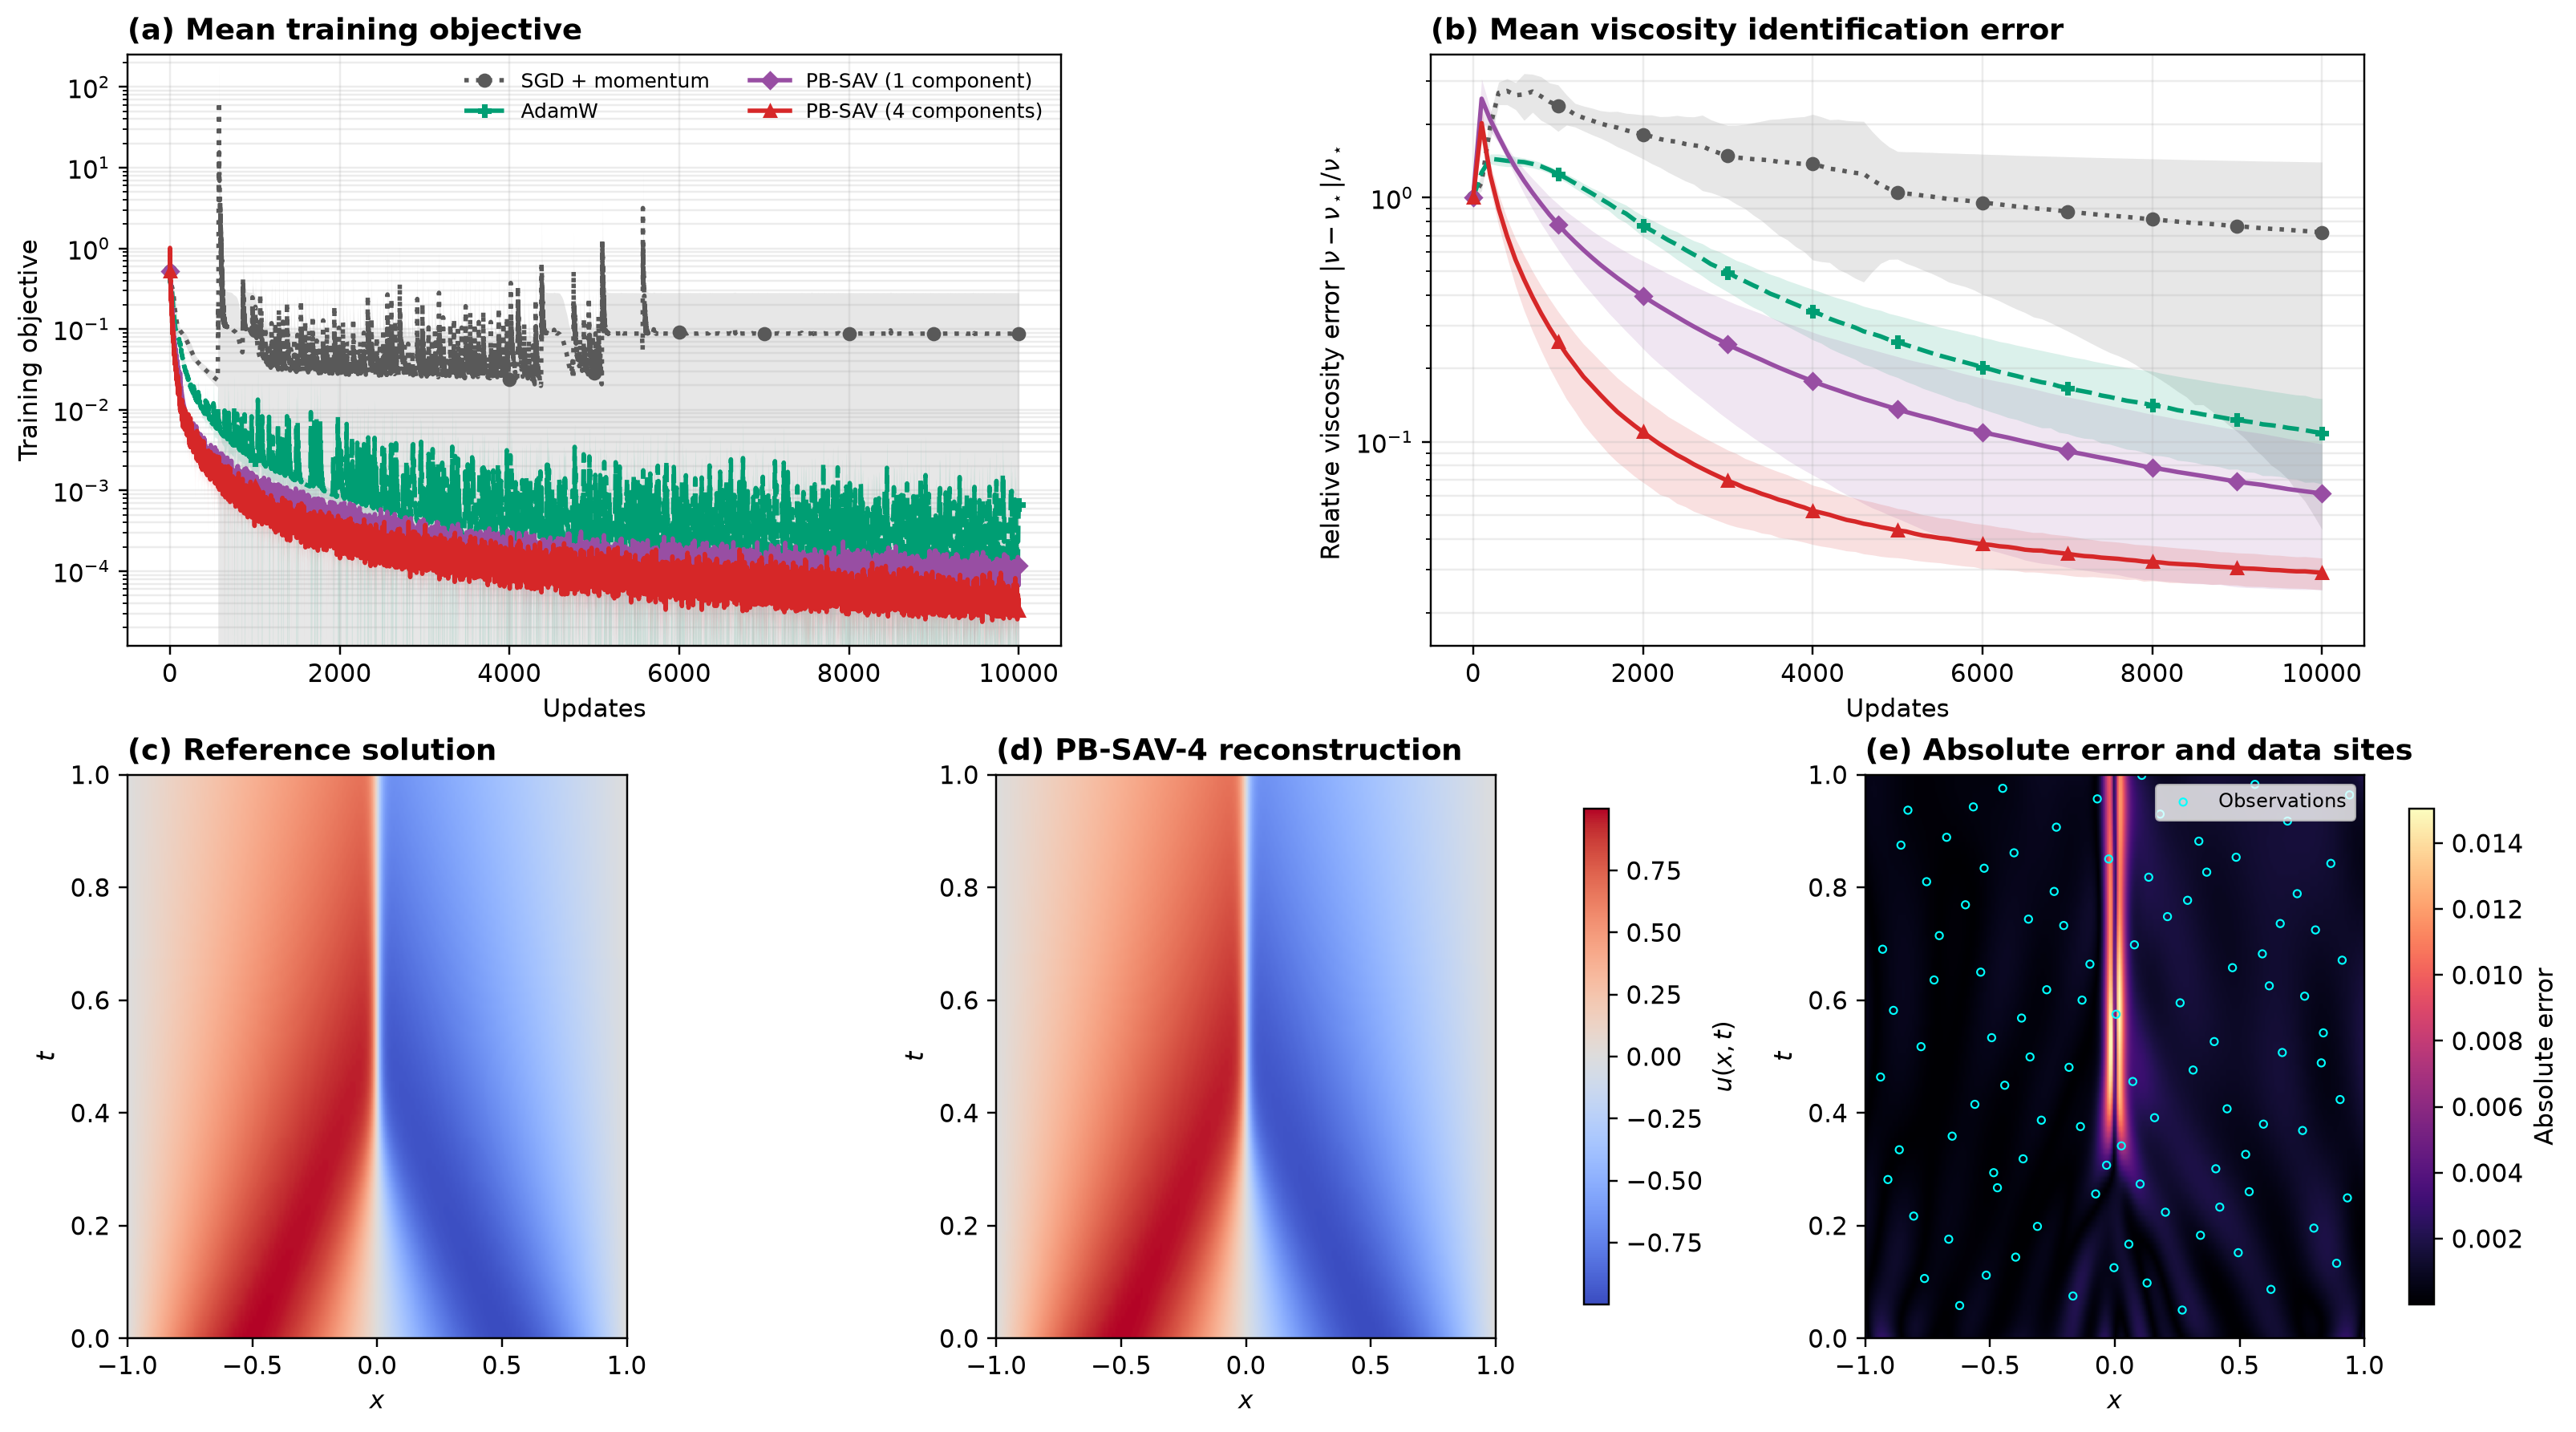
\includegraphics[width=\textwidth]{burgers_inverse_comparison.png}
  \caption{Five-seed comparison for inverse Burgers identification.  (a) Mean
  common task objective and (b) mean relative viscosity error; shaded regions
  show one sample standard deviation.  The lower row uses seed 42, the median
  four-component PB--SAV seed according to final viscosity error: (c) reference
  solution, (d) four-component PB--SAV reconstruction, and (e) absolute error
  with the 100 observation
  locations.}
  \label{fig:burgers-inverse-results}
\end{figure}

\begin{table}[t]
\centering
\caption{Inverse Burgers results after 10,000 updates over five paired seeds.
Values are mean \(\pm\) sample standard deviation.  For each seed, the tail
task objective is averaged over the final 2,000 updates of \(F_{\rm inv}\).
Best mean values are bold.}
\label{tab:burgers-inverse-results}
\footnotesize
\setlength{\tabcolsep}{3pt}
\begin{tabular}{lcc}
\toprule
Method & \(\eta\) & \shortstack{Tail task\\objective} \\
\midrule
Heavy-ball GD & 0.01 & \((0.878\pm1.900)\times10^{-1}\) \\
AdamW & 0.001 & \((3.515\pm0.330)\times10^{-4}\) \\
PB--SAV (1 component) & 0.003 & \((9.507\pm2.000)\times10^{-5}\) \\
PB--SAV (4 components) & 0.01 & \(\mathbf{(4.816\pm2.000)\times10^{-5}}\) \\
\bottomrule
\end{tabular}

\medskip
\begin{tabular}{lcc}
\toprule
Method & \shortstack{Final viscosity\\relative error} &
\shortstack{Final relative\\\(L^2\) error} \\
\midrule
Heavy-ball GD & \((7.213\pm6.800)\times10^{-1}\) & \((2.293\pm4.300)\times10^{-1}\) \\
AdamW & \((1.088\pm0.420)\times10^{-1}\) & \((1.440\pm0.650)\times10^{-2}\) \\
PB--SAV (1 component) & \((6.141\pm3.700)\times10^{-2}\) & \((7.476\pm3.300)\times10^{-3}\) \\
PB--SAV (4 components) & \(\mathbf{(2.914\pm0.430)\times10^{-2}}\) & \(\mathbf{(3.356\pm0.310)\times10^{-3}}\) \\
\bottomrule
\end{tabular}
\end{table}

The mean wall times were \(404.8\pm9.2\), \(408.2\pm8.2\),
\(567.1\pm33.0\), and \(583.6\pm35.0\) seconds for heavy-ball gradient
descent, AdamW, one-component PB--SAV, and four-component PB--SAV,
respectively.  All four methods use \(\lambda=3\times10^{-7}\).

Four-component PB--SAV gives the best mean result for the training objective,
viscosity identification, and solution reconstruction in
\cref{fig:burgers-inverse-results,tab:burgers-inverse-results}.  Relative to
one-component PB--SAV at its own selected learning rate, it reduces the mean
tail objective by 49.3\%, the mean viscosity error by 52.5\%, and the mean
solution error by 55.1\%.  Its solution-error standard deviation is
approximately 10.6 times smaller, and its viscosity-error standard deviation
is approximately 8.6 times smaller.
Relative to AdamW, the mean reductions in these three quantities are 86.3\%,
73.2\%, and 76.7\%, respectively.  The four-component method is 2.9\% slower
than one-component PB--SAV in the recorded wall time and 43.0\% slower than
AdamW.

Heavy-ball gradient descent converges to a near-zero field on seed 2669,
which accounts for the large mean and variance in its aggregate row.  AdamW
approaches the viscosity on all five seeds, but its task objective exhibits
large late spikes.

The representative reconstruction in \cref{fig:burgers-inverse-results}
tracks the reference solution throughout most of the space--time domain.  The
largest remaining error occurs near the steep central layer, where the
solution is most sensitive to viscosity. The four-component optimizer attains
lower mean errors at its selected learning rate with a small additional cost
over one-component PB--SAV; the forward experiment compares the pullbacks at a
common learning rate.

\FloatBarrier
